\subsection{CSS}

\begin{figure}[H]
			\centering
			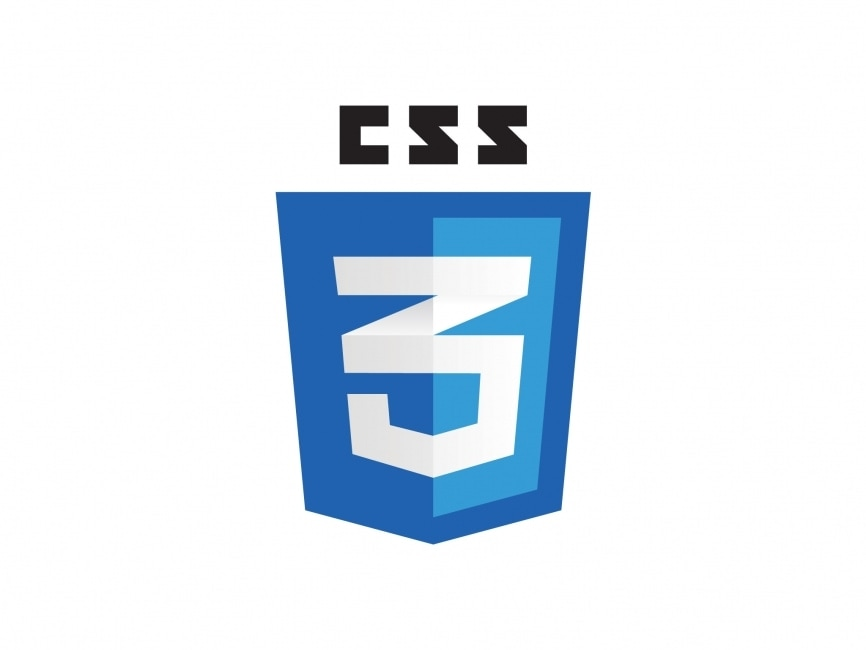
\includegraphics[scale=0.3]{./3_Stand_der_Technik/Abbildungen/CSS_LOGO}
			\caption{CSS-Logo \cite{Wikipedia2024d}}
		\end{figure}

CSS, oder Cascading Style Sheets, ist eine Stylesheet-Sprache, die verwendet wird, um das Aussehen und die Formatierung von Webseiten zu definieren. Mit CSS k�nnen Entwickler das Layout, die Farben, Schriftarten und andere visuelle Aspekte einer Webseite gestalten. Durch die Trennung von Inhalt und Darstellung erm�glicht CSS eine konsistente und effiziente Gestaltung von Webseiten. CSS wird zusammen mit HTML verwendet, um ansprechende und benutzerfreundliche Webseiten zu erstellen.


	\subsubsection{Syntax und Struktur von CSS-Regeln} 
CSS-Regeln bestehen aus einem Selektor und einer Deklaration.
Der Selektor w�hlt das HTML-Element aus, das gestylt werden soll.
Die Deklaration besteht aus Eigenschaften und Werten, die das Aussehen des ausgew�hlten Elements definieren.\cite{ionos.de2024}

	\subsubsection{Verwendung von Selektoren zur Gestaltung von HTML-Elementen} 
Selektoren identifizieren die HTML-Elemente, auf die die CSS-Stile angewendet werden sollen.
Es gibt verschiedene Arten von Selektoren, darunter Elementselektoren, Klassenselektoren, ID-Selektoren und kombinierte Selektoren.\cite{ionos.de2024}

	\subsubsection{Grundlegende Eigenschaften und Werte f�r die Gestaltung von Layout und Design} 
CSS bietet eine Vielzahl von Eigenschaften und Werten zur Gestaltung von Layout und Design, wie zum Beispiel color, font-size, margin, padding, background-color usw.
Diese Eigenschaften und Werte erm�glichen es Entwicklern, die Gr��e, Farbe, Schriftart, Abst�nde und Hintergr�nde von HTML-Elementen anzupassen.\cite{ionos.de2024}

	\subsubsection{Layout und Positionierung} 
Positionierung von Elementen auf der Seite:
CSS erm�glicht die Positionierung von Elementen auf einer Webseite relativ zum Bildschirm oder zu anderen Elementen.
Die Positionierung kann mithilfe von Eigenschaften wie position, top, bottom, left und right gesteuert werden.
Einfache Layouttechniken wie Flexbox oder Floats:
Flexbox ist eine CSS-Layout-Technik, die das Erstellen von flexiblen und responsiven Layouts erm�glicht. Sie erm�glicht das einfache Anordnen von Elementen in einer Zeile oder Spalte und die dynamische Anpassung der Gr��e und Reihenfolge.
Floats sind eine �ltere Layout-Technik, die verwendet werden kann, um Elemente zu einem bestimmten Bereich zu verschieben und den Textfluss um sie herum zu steuern. Sie werden oft f�r das Erstellen von Spaltenlayouts verwendet, obwohl Flexbox jetzt oft bevorzugt wird.
Diese einfachen Layout-Techniken erm�glichen es Entwicklern, das Design und die Anordnung von Elementen auf Webseiten zu steuern und ansprechende Layouts zu erstellen.\cite{ionos.de2024}

	\subsubsection{Stilisierung von Elementen} 
Anpassung von Farben, Schriftarten und Hintergr�nden:
Mit CSS k�nnen Farben, Schriftarten und Hintergr�nde von HTML-Elementen angepasst werden, um das Aussehen der Webseite zu verbessern.
Die Eigenschaften color, font-family, background-color und background-image sind einige Beispiele f�r Stileigenschaften, die verwendet werden k�nnen.
Einfache Animationen und �berg�nge:
CSS erm�glicht es, Elemente auf der Seite zu animieren oder �berg�nge zwischen Zust�nden zu erstellen, um eine ansprechendere Benutzererfahrung zu schaffen.
Die animation- und transition-Eigenschaften werden verwendet, um einfache Animationen und �berg�nge zu definieren, wie z.B. das Verschieben, Drehen oder Verblassen von Elementen.\cite{ionos.de2024}

	\subsubsection{Responsives Design} 
Grundlegende Anpassung des Layouts an verschiedene Bildschirmgr��en:
Responsives Design passt das Layout einer Webseite automatisch an verschiedene Bildschirmgr��en an.
Media Queries erm�glichen es, CSS-Regeln basierend auf den Eigenschaften des Ger�ts zu definieren.
Flexible Einheiten wie Prozentangaben oder relative Einheiten erm�glichen eine skalierbare Gestaltung.
Elemente k�nnen je nach Bildschirmgr��e angezeigt, ausgeblendet oder umgestaltet werden.\cite{ionos.de2024}


	\subsubsection{Zusammenfassung und Zukunft} 
Zusammenfassung der wichtigsten CSS-Konzepte f�r die Telemetrie-Website:
Grundlegende CSS-Konzepte wie Layout, Stilisierung von Elementen und responsives Design wurden angewendet.
M�gliche Erweiterungen und Optimierungen f�r zuk�nftige Entwicklungen:
Fortgeschrittenere CSS-Techniken wie Grid Layouts k�nnten f�r komplexere Layouts verwendet werden.
Optimierung des CSS-Codes durch B�ndelung und Minifizierung f�r verbesserte Ladezeiten.\cite{ionos.de2024}
